\chapter{A planta domesticada}\label{ch:g12:domesticated-plants}

Ao lado de uma espiga moderna de milho --- seiscentos grãos em fileiras
bem arrumadas, embrulhados em palha, presos num sabugo que não os
solta --- estava a espiga do teosinto, a gramínea silvestre de que ela
veio: uma dúzia de grãos numa fileira só, cada um encerrado numa casca
pétrea, caindo um a um na maturação. Nove mil anos de escolha, por
agricultores que guardavam as sementes das plantas que preferiam,
transformaram uma na outra. O resultado não sobrevive a uma temporada
sem nós: uma espiga de milho deixada num campo apodrece onde está. Este
capítulo é sobre o que acontece com uma planta quando as pessoas viram
o ambiente que a seleciona --- e sobre os modos mais novos de mudar de
propósito os \omterm{def:g10:universal-dna:gene}{genes} de uma planta.

\section{A seleção pelas pessoas}

\begin{definition}[Domesticação, seleção artificial]\label{def:g12:domesticated-plants:domestication}
A \emph{domesticação}\index{domesticação} é a transformação de uma
\omterm{def:g10:biodiversity-scales:species}{espécie} silvestre numa que depende dos seres humanos e os serve, pela
\emph{seleção artificial}\index{seleção artificial}: a cada geração, as
pessoas guardam e semeiam as sementes dos indivíduos com os caracteres
que elas querem, de modo que os \omterm{def:g10:universal-dna:gene}{alelos} por trás desses caracteres sobem
de frequência. É a seleção do
\cref{ch:g12:selection-drift-speciation} com um olho humano no lugar do
ambiente, e funciona pela mesma aritmética --- mais rápido, já que a
escolha é deliberada e severa.
\end{definition}

\begin{proposition}[O que a domesticação seleciona]\label{prop:g12:domesticated-plants:traits}
As culturas compartilham um conjunto de caracteres que planta silvestre
nenhuma conservaria, a \emph{síndrome de \omterm{def:g12:domesticated-plants:domestication}{domesticação}}: sementes que
ficam na planta em vez de se espalhar (uma espiga que não se desfaz);
sementes e frutos maiores; sementes que germinam de imediato em vez de
esperar anos no solo; a perda das toxinas e das defesas amargas; uma
planta compacta, com poucos ramos e uma espiga grande em vez de muitas
pequenas; e amadurecimento simultâneo. Cada um é útil a quem colhe e
prejudicial a uma planta por conta própria --- uma cultura é uma planta
selecionada para a nossa conveniência e contra a independência dela.
\end{proposition}
\begin{proof}[Evidence]
O trigo silvestre solta os grãos de um eixo quebradiço; os primeiros
trigos cultivados, encontrados nos sítios agrícolas mais antigos, têm
um eixo resistente que segura o grão --- a foice de quem colhia
selecionou, sem querer, os mutantes cujo grão ficava na planta para ser
recolhido e semeado. O teosinto e o milho diferem em apenas cerca de
cinco \omterm{def:g10:universal-dna:gene}{genes} principais: um transforma uma planta muito ramificada num
caule único, outro solta o grão da casca pétrea dele, outros
multiplicam as fileiras. Cruzar os dois dá descendentes férteis, e as
formas intermediárias existem: a mesma \omterm{def:g10:biodiversity-scales:species}{espécie}, remodelada.
\end{proof}

\begin{omfigure}
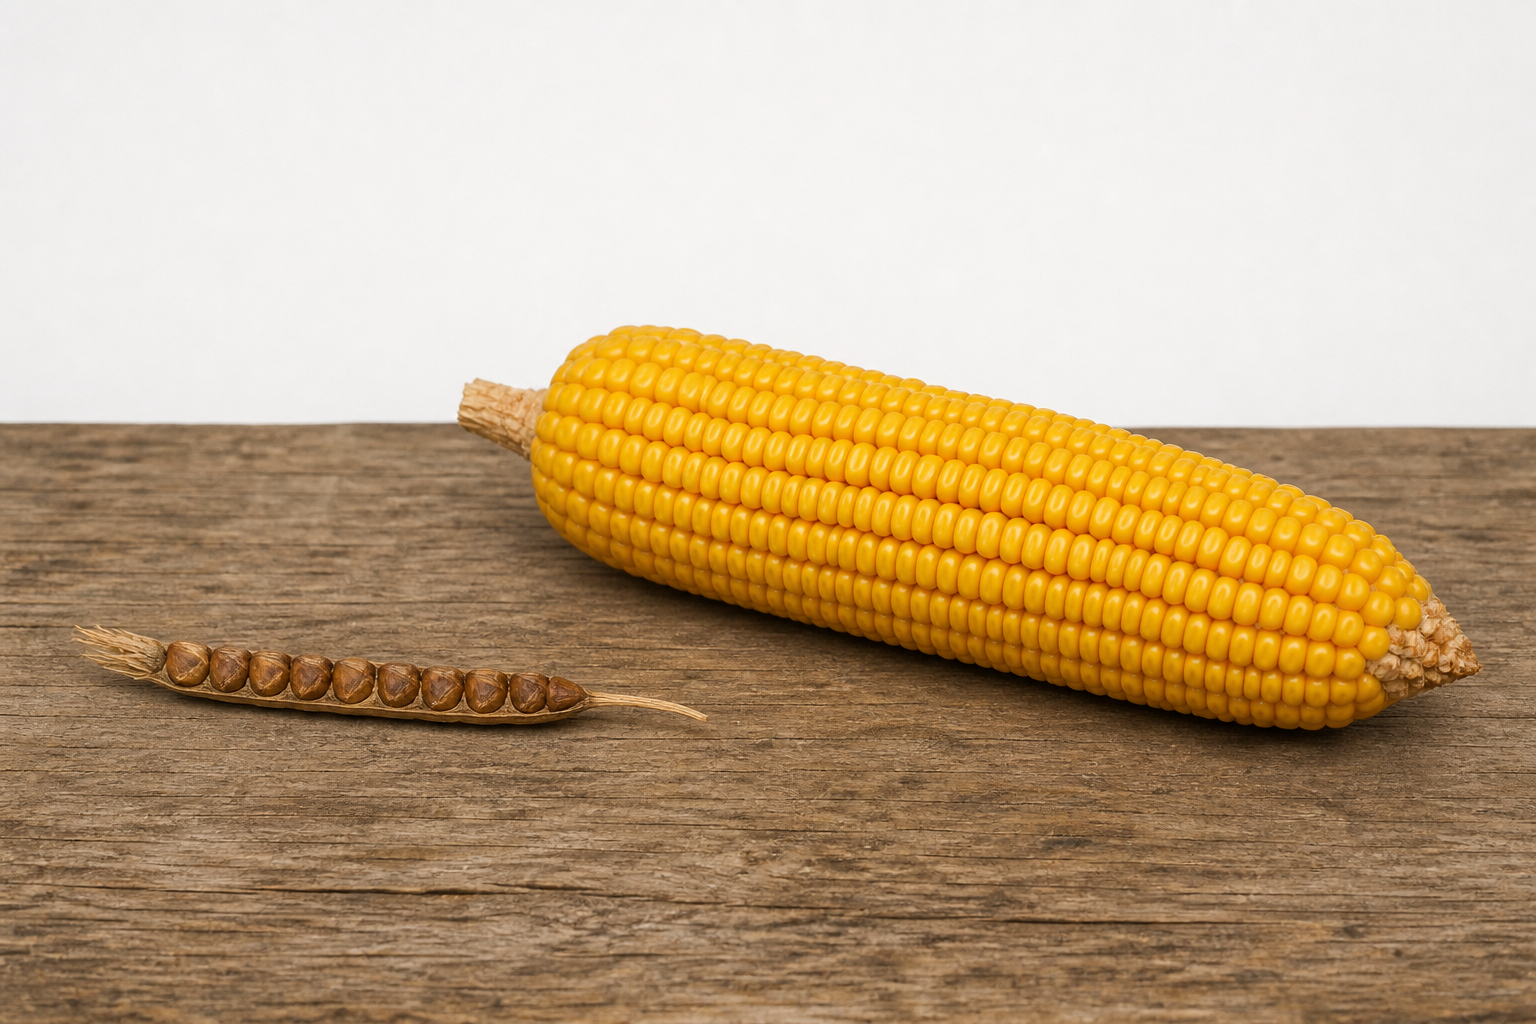
\includegraphics[width=0.62\linewidth]{images/book2/ai/g12-domestic-teosinte-maize.png}

{\small O teosinto e o milho. Uma dúzia de grãos encerrados numa fileira
só numa espiga quebradiça, contra centenas de grãos nus firmes num
sabugo: nove mil anos de escolha, e um punhado de \omterm{def:g10:universal-dna:gene}{genes}.}
\end{omfigure}

\begin{omfigure}
\begin{tikzpicture}[font=\small, >=Stealth,
  b/.style={draw, rounded corners, align=center, text width=2.2cm, minimum height=0.9cm}]
  \node[b, fill=omMeth!15, text width=2.8cm] (wild) at (0,0) {couve silvestre\\ (uma espécie)};
  \node[b, fill=omDef!12] (kale) at (5,3.0) {couve:\\ folhas};
  \node[b, fill=omDef!12] (cab) at (5,1.8) {repolho:\\ gema terminal};
  \node[b, fill=omDef!12, text width=2.7cm] (spr) at (5,0.6) {couve-de-bruxelas:\\ gemas laterais};
  \node[b, fill=omDef!12] (kohl) at (5,-0.6) {couve-rábano:\\ caule};
  \node[b, fill=omDef!12] (broc) at (5,-1.8) {brócolis:\\ botões florais};
  \node[b, fill=omDef!12] (cauli) at (5,-3.0) {couve-flor:\\ pedúnculos florais};
  \foreach \t in {kale,cab,spr,kohl,broc,cauli} \draw[->] (wild.east) -- (\t.west);
  \node[anchor=west, align=left, text width=4.6cm] at (7.2,0) {Seis culturas, uma espécie: em cada linhagem os agricultores selecionaram o exagero de um órgão diferente. As seis ainda se cruzam.};
\end{tikzpicture}

{\small A \omterm{def:g12:domesticated-plants:domestication}{seleção artificial} a partir de uma \omterm{def:g10:biodiversity-scales:species}{espécie} silvestre.
Selecionar folhas, gemas, caule ou flores em linhagens diferentes
produziu plantas que parecem \omterm{def:g10:biodiversity-scales:species}{espécies} diferentes e não são.}
\end{omfigure}

\begin{example}[O que uma cultura perdeu]\label{ex:g12:domesticated-plants:lost}
O milho não consegue espalhar a semente dele; o trigo cultivado não
consegue soltar o grão dele; a banana e a uva sem semente não fazem
semente nenhuma e são propagadas por estacas, cada planta um clone. A
sobrevivência de uma cultura é delegada ao agricultor, e a
\emph{\omterm{def:g10:biodiversity-scales:biodiversity}{diversidade genética}} dela encolheu a cada etapa de seleção: uma
variedade moderna é quase uniforme, e uma região inteira pode cultivar
uma só. Os parentes silvestres, ainda diversos, são onde ficam
guardados os \omterm{def:g10:universal-dna:gene}{alelos} de que uma cultura futura pode precisar --- para
uma doença nova, um clima mais seco (\cref{ch:g10:biodiversity-scales}).
\end{example}

\section{O melhoramento por cruzamento}

\begin{proposition}[Variedades e híbridos]\label{prop:g12:domesticated-plants:hybrids}
Os melhoristas fazem variedades novas cruzando plantas que carregam
\omterm{def:g10:universal-dna:gene}{alelos} úteis diferentes e selecionando, entre os descendentes, as
combinações que querem, ao longo de várias gerações. Um caso especial
domina o milho e muitas hortaliças: o \emph{híbrido F1}\index{híbrido
F1}. Duas linhagens endogâmicas --- cada uma tornada uniforme e
homozigota por gerações de autopolinização --- são cruzadas; os
descendentes delas são todos geneticamente idênticos, heterozigotos em
cada \omterm{def:g10:universal-dna:gene}{gene} em que as linhagens diferem, e nitidamente mais vigorosos e
produtivos que qualquer um dos genitores. Semeada de novo, a própria
semente do híbrido segrega numa mistura de plantas menos vigorosas: o
agricultor compra semente híbrida nova todo ano.
\end{proposition}
\admitted

\begin{omfigure}
\begin{tikzpicture}[font=\small, >=Stealth,
  b/.style={draw, rounded corners, align=center, text width=2.6cm, minimum height=1.0cm}]
  \node[b, fill=omDef!12] (a) at (0,1.2) {linhagem endogâmica A\\ $AA\,bb$, uniforme};
  \node[b, fill=omDef!12] (bb) at (0,-1.2) {linhagem endogâmica B\\ $aa\,BB$, uniforme};
  \node[b, fill=omMeth!20, text width=3.0cm] (f1) at (4.6,0) {híbrido F1\\ $Aa\,Bb$, todos idênticos,\\ vigorosos};
  \node[b, fill=omProp!15, text width=3.4cm] (f2) at (9.6,0) {F2 da semente do híbrido:\\ $AA$, $Aa$, $aa$ \dots misturados,\\ 15--20\% menos produtivos};
  \draw[->] (a) -- (f1); \draw[->] (bb) -- (f1);
  \draw[->] (f1) -- node[above] {semeado de si mesmo} (f2);
\end{tikzpicture}

{\small O \omterm{prop:g12:domesticated-plants:hybrids}{híbrido F1}. Duas linhagens homozigotas dão descendentes
heterozigotos uniformes de alto vigor; a geração seguinte segrega e o
perde, e assim a semente precisa ser comprada de novo a cada ano --- a
base da indústria de sementes.}
\end{omfigure}

\begin{omfigure}
\begin{tikzpicture}
\begin{axis}[
  width=0.86\linewidth, height=5.6cm,
  axis x line=bottom, axis y line=left,
  xmin=1900, xmax=2025, ymin=0, ymax=9,
  xlabel={ano}, ylabel={produtividade do trigo (t/ha)},
  xlabel style={font=\small, at={(axis description cs:0.5,-0.12)}, anchor=north},
  ylabel style={font=\small},
  tick label style={font=\small}, xtick={1900,1925,1950,1975,2000,2025}, ytick={0,2,4,6,8},
  clip=false,
]
\addplot[thick, omMeth, mark=*, mark size=1.5pt] coordinates
  {(1900,1.3) (1920,1.4) (1940,1.6) (1950,1.9) (1960,2.6) (1970,3.6) (1980,5.0) (1990,6.5) (2000,7.2) (2010,7.3) (2020,7.5)};
\draw[dashed, gray] (axis cs:1955,0) -- (axis cs:1955,8.5);
\node[font=\scriptsize, anchor=south, align=center] at (axis cs:1955,8.5) {variedades de colmo curto,\\ fertilizante, pesticidas};
\end{axis}
\end{tikzpicture}

{\small Produtividade média do trigo num país da Europa ocidental ao
longo de um século (arredondada). Estável por cinquenta anos, depois
quadruplicada em quarenta por variedades novas melhoradas para carregar
espigas pesadas em colmos curtos, junto com fertilizante e controle de
pragas. O patamar desde 2000 é o assunto do melhoramento atual.}
\end{omfigure}

\begin{example}[Por que o híbrido é vigoroso, e por que isso não dura]\label{ex:g12:domesticated-plants:vigour}
Cada linhagem endogâmica, homozigota em toda parte, carrega alguns
\omterm{def:g10:universal-dna:gene}{alelos} \omterm{def:g11:genes-and-disease:genetic}{recessivos} fracos em dose dupla; cruzar duas linhagens mascara
os \omterm{def:g10:universal-dna:gene}{alelos} fracos de cada uma atrás dos \omterm{def:g10:universal-dna:gene}{alelos} funcionais da outra, em
cada \omterm{def:g10:universal-dna:gene}{gene} em que elas diferem. A F1 é, portanto, heterozigota e
vigorosa. Na geração seguinte, a \omterm{def:g12:meiosis-genetic-shuffling:meiosis}{meiose} e a fecundação distribuem os
\omterm{def:g10:universal-dna:gene}{alelos} de novo (\cref{ch:g12:meiosis-genetic-shuffling}): um quarto das
plantas é homozigoto para o \omterm{def:g10:universal-dna:gene}{alelo} fraco em cada \omterm{def:g10:universal-dna:gene}{gene}, e o campo vira
uma colcha de retalhos.
\end{example}

\section{Mudar os genes diretamente}

\begin{proposition}[Culturas transgênicas e editadas]\label{prop:g12:domesticated-plants:transgenic}
Desde os anos 1980 um \omterm{def:g10:universal-dna:gene}{gene} pode ser introduzido numa planta sem
cruzamento: a \emph{transgênese}\index{transgênese}
(\cref{ch:g10:universal-dna}). Uma bactéria do solo que naturalmente
injeta um pedaço do \omterm{def:g10:universal-dna:information}{DNA} dela nas \omterm{def:g10:cells-common-unit:cell}{células} vegetais é usada como veículo:
o \omterm{def:g10:universal-dna:gene}{gene} desejado é inserido nesse pedaço, \omterm{def:g10:cells-common-unit:cell}{células} vegetais são
infectadas, e plantas inteiras são regeneradas a partir das \omterm{def:g10:cells-common-unit:cell}{células} que
receberam o \omterm{def:g10:universal-dna:gene}{gene}. O \omterm{def:g10:universal-dna:gene}{gene} pode vir de qualquer \omterm{def:g10:biodiversity-scales:species}{espécie}. Mais
recentemente, os próprios \omterm{def:g10:universal-dna:gene}{genes} de uma planta podem ser alterados numa
posição escolhida --- a \emph{edição gênica} --- sem acrescentar \omterm{def:g10:universal-dna:information}{DNA}
estranho. Caracteres até agora: resistência a um inseto (um \omterm{def:g10:universal-dna:gene}{gene} de
toxina bacteriana), tolerância a um herbicida, resistência a um vírus,
um precursor de vitamina no arroz, óleos de composição alterada.
\end{proposition}
\admitted

\begin{omfigure}
\begin{tikzpicture}[font=\small, >=Stealth,
  b/.style={draw, rounded corners, align=center, text width=2.4cm, minimum height=1.0cm}]
  \node[b, fill=omThm!12] (gene) at (0,0) {gene de interesse\\ (qualquer espécie)};
  \node[b, fill=omProp!15] (bact) at (3.3,0) {inserido no DNA que\\ uma bactéria do solo\\ transfere às plantas};
  \node[b, fill=omDef!12] (cells) at (6.6,0) {células vegetais infectadas;\\ algumas incorporam\\ o gene};
  \node[b, fill=omMeth!15] (plant) at (9.9,0) {plantas inteiras regeneradas\\ dessas células:\\ transgênicas};
  \draw[->] (gene) -- (bact); \draw[->] (bact) -- (cells); \draw[->] (cells) -- (plant);
\end{tikzpicture}

{\small Fazer uma planta transgênica. Uma bactéria que naturalmente
insere \omterm{def:g10:universal-dna:information}{DNA} nas \omterm{def:g10:cells-common-unit:cell}{células} vegetais leva o \omterm{def:g10:universal-dna:gene}{gene} escolhido para dentro; as
plantas são regeneradas a partir das \omterm{def:g10:cells-common-unit:cell}{células} que o receberam, e o
transmitem pelas sementes delas.}
\end{omfigure}

\begin{example}[Um gene de toxina no milho]\label{ex:g12:domesticated-plants:bt}
Uma bactéria do solo fabrica uma \omterm{def:g11:gene-expression:protein}{proteína} tóxica para as lagartas e
inofensiva para os mamíferos; o \omterm{def:g10:universal-dna:gene}{gene} dela, inserido no milho, faz cada
\omterm{def:g10:cells-common-unit:cell}{célula} da planta produzir a toxina, e as lagartas da broca que fazem
túneis nos colmos morrem na primeira mordida. A pulverização de
inseticida cai; as produtividades sobem onde a broca era severa. Em uma
década, brocas resistentes à toxina apareceram onde a cultura era
plantada sem interrupção --- a seleção do
\cref{ch:g11:antibiotic-resistance} num campo --- e os agricultores
hoje são obrigados a semear refúgios de milho comum ao lado do
transgênico, para que brocas sensíveis sobrevivam e diluam as resistentes.
\end{example}

\section{Escolhas}

\begin{proposition}[O que está em jogo]\label{prop:g12:domesticated-plants:stakes}
Toda técnica deste capítulo levanta as mesmas questões numa forma nova:
o estreitamento da diversidade (uma variedade numa região inteira, um
\omterm{def:g10:universal-dna:gene}{gene} em cada planta), a dependência dos agricultores em relação a uma
semente que eles não podem guardar, a seleção de pragas e ervas
daninhas resistentes às defesas da cultura, a passagem dos \omterm{def:g10:universal-dna:gene}{genes} de uma
cultura aos parentes silvestres pelo pólen, e a segurança e a
propriedade do que se come. Nenhuma delas é respondida só pela
biologia; a biologia diz o que cada técnica faz e não faz, e o que ela seleciona.
\end{proposition}
\admitted

\begin{method}[Ler a história de uma cultura]\label{met:g12:domesticated-plants:read}
\begin{enumerate}
  \item Identifique o ancestral silvestre e o que a cultura perdeu em
        relação a ele (dispersão, dormência, defesas, diversidade).
  \item Identifique como a mudança foi feita: seleção inconsciente pela
        colheita, seleção deliberada, cruzamento e seleção, hibridação,
        \omterm{prop:g10:universal-dna:universal}{transgênese}, edição.
  \item Conte os \omterm{def:g10:universal-dna:gene}{genes} envolvidos onde eles são conhecidos: poucos
        \omterm{def:g10:universal-dna:gene}{genes} principais para a síndrome de \omterm{def:g12:domesticated-plants:domestication}{domesticação}, muitos \omterm{def:g10:universal-dna:gene}{genes}
        pequenos para a produtividade, um para um caráter transgênico.
  \item Pergunte de que a cultura depende hoje (o agricultor, a semente
        comprada, um herbicida, os refúgios) e o que depende dela.
\end{enumerate}
\end{method}

\begin{remark}[O experimento mais antigo em evolução]\label{rem:g12:domesticated-plants:oldest}
Darwin abriu o livro dele sobre a origem das \omterm{def:g10:biodiversity-scales:species}{espécies} com um capítulo
sobre pombos e couves, porque os criadores já tinham mostrado o que a
seleção conseguia fazer em alguns séculos; ele só precisou tirar o
criador e alongar o tempo. Toda cultura é uma demonstração dos três
últimos capítulos --- variação, seleção e uma mudança de frequências
que altera uma \omterm{def:g10:biodiversity-scales:species}{espécie} --- rodada na velocidade humana, com um registro
dos resultados em cada campo e em cada feira.
\end{remark}

\section{Exercícios}

\begin{exercise}[$\star$]\label{exo:g12:domesticated-plants:1}
Defina \omterm{def:g12:domesticated-plants:domestication}{domesticação} e \omterm{def:g12:domesticated-plants:domestication}{seleção artificial}.
\end{exercise}

\begin{exercise}[$\star$]\label{exo:g12:domesticated-plants:2}
Liste quatro caracteres da síndrome de \omterm{def:g12:domesticated-plants:domestication}{domesticação} e diga por que cada
um é uma desvantagem para uma planta silvestre.
\end{exercise}

\begin{exercise}[$\star$]\label{exo:g12:domesticated-plants:3}
O que é um \omterm{prop:g12:domesticated-plants:hybrids}{híbrido F1}, e por que os agricultores compram a semente dele todo ano?
\end{exercise}

\begin{exercise}[$\star$]\label{exo:g12:domesticated-plants:4}
Como um \omterm{def:g10:universal-dna:gene}{gene} é introduzido numa planta sem cruzamento?
\end{exercise}

\begin{exercise}[$\star$]\label{exo:g12:domesticated-plants:5}
A partir da figura da produtividade, em que fator a produtividade do
trigo subiu entre 1950 e 2000?
\end{exercise}

\begin{exercise}[$\star\star$]\label{exo:g12:domesticated-plants:6}
Explique como a colheita com uma foice, sem intenção nenhuma de
melhoramento, selecionou o trigo de eixo resistente.
\end{exercise}

\begin{exercise}[$\star\star$]\label{exo:g12:domesticated-plants:7}
A couve, o repolho e o brócolis se cruzam livremente. Eles são uma
\omterm{def:g10:biodiversity-scales:species}{espécie} ou três? O que os deixou tão diferentes?
\end{exercise}

\begin{exercise}[$\star\star$]\label{exo:g12:domesticated-plants:8}
Duas linhagens endogâmicas são cruzadas. Num \omterm{def:g10:universal-dna:gene}{gene} em que a linhagem A é
$AA$ e a linhagem B é $aa$, dê o \omterm{def:g11:enzymes-and-phenotype:phenotype}{genótipo} da F1 e os \omterm{def:g11:enzymes-and-phenotype:phenotype}{genótipos} e as
proporções da F2. Por que a F1 é uniforme e a F2 não?
\end{exercise}

\begin{exercise}[$\star\star$]\label{exo:g12:domesticated-plants:9}
Por que brocas resistentes apareceram em campos de milho produtor de
toxina, e como um refúgio de milho comum as retarda?
\end{exercise}

\begin{exercise}[$\star\star$]\label{exo:g12:domesticated-plants:10}
O teosinto e o milho diferem em cerca de cinco \omterm{def:g10:universal-dna:gene}{genes} principais.
Explique como tão poucos \omterm{def:g10:universal-dna:gene}{genes} conseguem mudar tanto a planta, usando o
\cref{ch:g12:diversification-of-life}.
\end{exercise}

\begin{exercise}[$\star\star$]\label{exo:g12:domesticated-plants:11}
Por que os parentes silvestres das culturas são conservados em bancos
de sementes, se eles quase não produzem nada?
\end{exercise}

\begin{exercise}[$\star\star\star$]\label{exo:g12:domesticated-plants:12}
Uma colza tolerante a herbicida é cultivada ao lado de uma mostarda
silvestre com a qual ela consegue se cruzar. Preveja o que pode
acontecer ao longo de alguns anos, e nomeie os processos dos capítulos
anteriores envolvidos.
\end{exercise}

\begin{exercise}[$\star\star\star$]\label{exo:g12:domesticated-plants:13}
A curva da produtividade está estável desde 2000. Proponha duas razões
biológicas e uma não biológica, e diga o que um melhorista poderia tentar.
\end{exercise}

\begin{exercise}[$\star\star\star$]\label{exo:g12:domesticated-plants:14}
Compare, em três pontos, uma variedade obtida por cruzamento e seleção
com uma obtida por \omterm{prop:g10:universal-dna:universal}{transgênese}: a origem do \omterm{def:g10:universal-dna:gene}{alelo} novo, o número de
\omterm{def:g10:universal-dna:gene}{genes} mudados e o tempo levado.
\end{exercise}

\begin{exercise}[$\star\star\star$]\label{exo:g12:domesticated-plants:15}
``A \omterm{def:g12:domesticated-plants:domestication}{domesticação} é o contrário da \omterm{def:g12:selection-drift-speciation:selection}{seleção natural}.'' Discuta num
parágrafo com a aritmética das \omterm{def:g12:selection-drift-speciation:population}{frequências alélicas}, o agente da
seleção e o destino da planta selecionada.
\end{exercise}

\section{Problema: nove mil anos, cinco genes}

\begin{problem}[{Problema de fim de semana --- o milho feito a partir
do teosinto: as espigas comparadas, a seleção contabilizada, a
produtividade de um híbrido acompanhada até a F2, e um gene de toxina
manejado contra a resistência}]
\label{pb:g12:domesticated-plants:1}
Uma espiga de teosinto carrega 12 grãos de \qty{0.08}{g}, encerrados
numa casca dura, num eixo quebradiço; uma espiga de milho carrega 600
grãos de \qty{0.3}{g}, nus, num sabugo rígido. O milho foi domesticado
há cerca de 9000 anos; uma geração é um ano.

\medskip
\noindent\textbf{Parte I --- As espigas.}
\begin{enumerate}
  \item Calcule a massa de grão por espiga no teosinto e no milho, e o
        fator entre as duas.
  \item Liste os caracteres da espiga de milho que pertencem à síndrome
        de \omterm{def:g12:domesticated-plants:domestication}{domesticação} e, para cada um, diga por que ele seria uma
        desvantagem para uma planta silvestre.
  \item O grão encerrado é controlado por um \omterm{def:g10:universal-dna:gene}{gene}, com o \omterm{def:g10:universal-dna:gene}{alelo} do grão
        nu \omterm{def:g11:genes-and-disease:genetic}{recessivo}. Explique por que os primeiros agricultores só
        poderiam ter encontrado plantas de grão nu como indivíduos
        raros nos campos deles.
  \item Suponha que o \omterm{def:g10:universal-dna:gene}{alelo} do grão nu tivesse frequência 0.01 na
        \omterm{def:g12:selection-drift-speciation:population}{população} silvestre. Que fração das plantas apresentava grãos nus?
  \item Uma agricultora semeia apenas semente de plantas de grão nu.
        Qual é a frequência do \omterm{def:g10:universal-dna:gene}{alelo} do grão nu na safra seguinte dela?
\end{enumerate}

\medskip
\noindent\textbf{Parte II --- Nove mil gerações.}
\begin{enumerate}[resume]
  \item O número de grãos da espiga subiu de 12 para 600 ao longo de
        9000 gerações. Calcule o fator médio de aumento por geração.
        Por que uma mudança tão pequena por geração basta?
  \item O número de fileiras de grãos é controlado por muitos \omterm{def:g10:universal-dna:gene}{genes} de
        efeito pequeno. Explique por que um caráter desses responde à
        seleção aos poucos e por muito tempo, enquanto o caráter do
        grão encerrado mudou num passo só.
  \item O milho ainda se cruza com o teosinto e dá descendentes
        férteis. Eles são uma \omterm{def:g10:biodiversity-scales:species}{espécie}? O que a \omterm{def:g12:domesticated-plants:domestication}{domesticação} mudou e o
        que ela não mudou?
  \item Uma variedade moderna é geneticamente uniforme. Enuncie o risco
        que decorre disso, e o recurso que responde a ele.
  \item O milho não consegue dispersar as sementes dele. O que isso
        implica sobre a relação entre a planta e o agricultor, em
        termos de seleção?
\end{enumerate}

\medskip
\noindent\textbf{Parte III --- O híbrido.}
A linhagem endogâmica A produz \qty{5}{t/ha}, a linhagem B
\qty{5.5}{t/ha}, o \omterm{prop:g12:domesticated-plants:hybrids}{híbrido F1} delas \qty{10}{t/ha}; a F2 cultivada a
partir da semente do híbrido produz \qty{8.2}{t/ha}. A semente híbrida
custa o equivalente a \qty{0.4}{t/ha} de milho.
\begin{enumerate}[resume]
  \item Em que porcentagem a F1 supera o melhor genitor? Em que
        porcentagem a F2 fica abaixo da F1?
  \item Explique o vigor da F1 e a perda da F2 com os \omterm{def:g11:enzymes-and-phenotype:phenotype}{genótipos} do
        \cref{ex:g12:domesticated-plants:vigour}.
  \item Um agricultor hesita entre comprar semente híbrida a cada ano e
        guardar semente da F1. Compare as colheitas líquidas, e diga
        por que o negócio da empresa de sementes existe.
  \item Por que as linhagens endogâmicas não podem simplesmente ser
        vendidas aos agricultores para que eles mesmos façam o híbrido?
  \item O que o sistema dos híbridos fez com a \omterm{def:g10:biodiversity-scales:biodiversity}{diversidade genética} dos
        campos e com a independência do agricultor?
\end{enumerate}

\medskip
\noindent\textbf{Parte IV --- O \omterm{def:g10:universal-dna:gene}{gene} de toxina.}
Uma \omterm{def:g12:selection-drift-speciation:population}{população} de broca tem um \omterm{def:g10:universal-dna:gene}{alelo} de resistência na frequência 0.001,
\omterm{def:g11:genes-and-disease:genetic}{recessivo}; só as brocas $rr$ sobrevivem no milho com toxina.
\begin{enumerate}[resume]
  \item Que fração das brocas sobrevive num campo de milho com toxina
        no primeiro ano? Calcule a frequência de $r$ entre as sobreviventes.
  \item Explique por que, sem refúgios, a resistência se espalha em
        poucos anos, usando o caso dos \omterm{def:g11:antibiotic-resistance:antibiotic}{antibióticos} como modelo.
  \item Um refúgio de milho comum mantém uma \omterm{def:g12:selection-drift-speciation:population}{população} grande de brocas
        sensíveis viva ao lado do campo com toxina. Explique como isso
        mantém o \omterm{def:g10:universal-dna:gene}{alelo} de resistência raro, usando o \omterm{def:g11:enzymes-and-phenotype:phenotype}{genótipo} dos
        descendentes de uma sobrevivente resistente e de uma broca do refúgio.
  \item Compare o refúgio com o ``ciclo completo'' de \omterm{def:g11:antibiotic-resistance:antibiotic}{antibióticos}: o
        que é igual, o que é diferente?
  \item Enuncie o resultado: o fator pelo qual a \omterm{def:g12:domesticated-plants:domestication}{domesticação}
        multiplicou o grão de uma espiga, o número de \omterm{def:g10:universal-dna:gene}{genes} principais
        que isso exigiu, e a única dependência que ela criou.
\end{enumerate}
\end{problem}
